\documentclass{amsart}

% biber

\usepackage[english]{babel}
\usepackage[utf8]{inputenc}
\usepackage{graphicx}
\usepackage{mathtools}
\usepackage{amsthm}
\usepackage{thmtools,thm-restate}
\usepackage{amsfonts}
\usepackage{amssymb}
\usepackage{hyperref}
\usepackage[backend=biber,url=true,doi=true,eprint=false,style=alphabetic]{biblatex}
\usepackage{enumitem}
\usepackage[justification=centering,singlelinecheck=false]{caption}
\usepackage{indentfirst}
\usepackage{algorithm}
\usepackage{algpseudocode}
\usepackage{listings}
\usepackage[x11names, rgb]{xcolor}
\usepackage{tikz}
\usepackage{hyperref}
\usepackage{subcaption}
\usepackage{booktabs}
\usepackage{linegoal}
\usepackage{csquotes}
\usetikzlibrary{snakes,arrows,shapes}

\addbibresource{references.bib}

\makeatletter
\def\subsection{\@startsection{subsection}{3}%
  \z@{.5\linespacing\@plus.7\linespacing}{.1\linespacing}%
  {\normalfont}}
\makeatother

\makeatletter
\patchcmd{\@setauthors}{\MakeUppercase}{}{}{}
\makeatother

\DeclareMathOperator*{\argmin}{arg\,min}
\DeclareMathOperator*{\argmax}{arg\,max}
\DeclareMathOperator*{\Val}{\text{Val}}
\DeclareMathOperator*{\Ch}{\text{Ch}}
\DeclareMathOperator*{\Pa}{\text{Pa}}
\DeclareMathOperator*{\Sc}{\text{Sc}}
\newcommand{\ov}{\overline}
\newcommand{\region}{\mathcal}

\newcommand\defeq{\mathrel{\overset{\makebox[0pt]{\mbox{\normalfont\tiny\sffamily def}}}{=}}}

\newcommand{\algorithmautorefname}{Algorithm}
\algrenewcommand\algorithmicrequire{\textbf{Input}}
\algrenewcommand\algorithmicensure{\textbf{Output}}

\algnewcommand\algorithmicref{\textbf{Reference}}
\algnewcommand\Reference{\item[\algorithmicref]}
\algnewcommand\algorithmicred{\textbf{Reduction}}
\algnewcommand\Reduction{\item[\algorithmicred]}
\algnewcommand\algorithmicdesc{\textbf{Description}}
\algnewcommand\Description{\item[\algorithmicdesc]}
\algnewcommand\algorithmiccom{\textbf{Comment}}
\algnewcommand\Commentx{\item[\algorithmiccom]}

\algrenewcomment[1]{\hspace{0.25cm}\(\triangleright\) #1}
\algnewcommand{\LineComment}[1]{\State\,\(\triangleright\) #1}

\captionsetup[table]{labelsep=space}

\setlistdepth{9}
\newlist{deepitemize}{itemize}{9}
\setlist[deepitemize,1]{label=$\bullet$}
\setlist[deepitemize,2]{label=$\bullet$}
\setlist[deepitemize,3]{label=$\bullet$}
\setlist[deepitemize,4]{label=$\bullet$}
\setlist[deepitemize,5]{label=$\bullet$}
\setlist[deepitemize,6]{label=$\bullet$}
\setlist[deepitemize,7]{label=$\bullet$}
\setlist[deepitemize,8]{label=$\bullet$}
\setlist[deepitemize,9]{label=$\bullet$}

\theoremstyle{plain}

\newcounter{dummy-def}\numberwithin{dummy-def}{section}
\newtheorem{definition}[dummy-def]{Definition}
\newtheorem{theorem}{Theorem}
\newcounter{dummy-prop}\numberwithin{dummy-prop}{section}
\newtheorem{proposition}[dummy-prop]{Proposition}
\newcounter{dummy-corollary}\numberwithin{dummy-corollary}{section}
\newtheorem{corollary}[dummy-corollary]{Corollary}
\newtheorem{lemma}{Lemma}
\newcounter{dummy-ex}\numberwithin{dummy-ex}{section}
\newtheorem{exercise}[dummy-ex]{Exercise}
\newcounter{dummy-eg}\numberwithin{dummy-eg}{section}
\newtheorem{example}[dummy-eg]{Example}

\newcommand{\set}[1]{\mathbf{#1}}
\newcommand{\pr}{\mathbb{P}}
\newcommand{\eps}{\varepsilon}
\renewcommand{\implies}{\Rightarrow}

\newcommand{\bigo}{\mathcal{O}}
\newcommand{\verifier}{\mathcal{V}}
\newcommand{\p}{\text{P}}
\newcommand{\np}{\text{NP}}
\newcommand{\conp}{\text{co-NP}}
\newcommand{\true}{\text{true}}
\newcommand{\false}{\text{false}}

\setlength{\parskip}{1em}

\lstset{frameround=fttt,
	numbers=left,
	breaklines=true,
	keywordstyle=\bfseries,
	basicstyle=\ttfamily,
}

\newcommand{\code}[1]{\lstinline[mathescape=true]{#1}}
\newcommand{\mcode}[1]{\lstinline[mathescape]!#1!}
\newcommand{\dset}[1]{\mathcal{#1}}
\newcommand{\ddspn}[2]{\frac{\partial#1}{\partial#2}}
\newcommand{\iddspn}[2]{\partial#1/\partial#2}

\title{%
  \noindent\rule{13cm}{1.0pt}\\
  \vspace{0.2cm}
  A Polynomial-time Reduction of the 3-SAT to the Quadratic Congruence and other Related Problems
  \noindent\rule{13cm}{0.8pt}
}
\xdef\shorttitle{Quadratic congruence polynomial-time reduction}
\author[]{\normalsize Renato Lui Geh\\\small NUSP\@: 8536030\\\\Computational Number Theory
(MAC6927)\\Prof\@. Sinai Robins\\University of São Paulo\\}

\begin{document}

\begin{abstract}
  In this term paper for MAC6927 --- Computational Number Theory, we explore the history behind the
  quadratic congruence problem (QCP) and other related number theoric problems; show a
  polynomial-time reduction from the 3-SAT to the QCP quoting Adleman and Manders' 1978
  theorem~\cite{qcp2}, implying that quadratic congruence is NP-complete; and show some solved and
  unsolved problems in Number Theory that are directly (or indirectly) related to the QCP problem
  and its membership in NP\@.
  \vspace*{-3.5em}
\end{abstract}

\maketitle

\section{History}

German mathematician David Hilbert published in 1902~\cite{hilbert} a set of 23 unsolved problems
in mathematics he deemed to be the most important mathematical problems to be solved in the 20th
century. Since then 9 of them have been solved, 9 are considered partially resolved, three of them
are unsolved and two of them are considered too vague (as of the time the author is writing this
line and as far as the author is aware). Unsolved problems include the infamous Riemann Hypothesis
and an extension to the Kronecker-Weber Theorem. Amongst solved problems is the 10th Hilbert
problem.

\textbf{10th Hilbert Problem:} Given a diophantine equation with any number of unknown quantities
and with rational integral numerical coefficients: \textit{to devise a process according to which
it can be determined by a finite number of operations whether the equation is solvable in rational
integers}.

It was answered in 1970 by Matiyasevich to be impossible~\cite{diophantine}. The question now
becomes, in which cases is there an algorithm for solvability and what is the complexity of such
algorithm? In 1976, Adleman and Manders~\cite{qcp1} partially answered these questions by proving
that, for the quadratic case, there exists an algorithm and the problem of finding the solutions is
NP-complete. In their proof, they also found that, through a slight modification in the final step
of their proof, it was possible to answer the quadratic congruence problem. A cleaner version of
this proof was published in 1978 by Adleman and Manders~\cite{qcp2}, proof we try to explain in
this paper.

In this paper we focus on the second result of Adleman and Manders' 1978 article (namely that the
quadratic congruence problem is NP-complete), but also briefly show the main result, i.e\ that
the set of quadratic diophantine equations with natural numbers solutions is NP-complete. The proof
is done through a polynomial-time reduction from the 3-SAT problem. This reduction implies that
both problems covered in Adleman and Manders' article are NP-complete.

In 1971, American mathematician Stephen Cook published ``The Complexity of Theorem-proving
Procedures''~\cite{cook}, and in the next year, his fellow countryman Richard Karp published
``Reducibility Among Combinatorial Problems''~\cite{karp}. The two articles introduced the concepts
of P and NP classes, yielding the duo a Turing Award. Interestingly in 1973, on the other side of
the Iron Curtain, Ukrainian Leonard Levin published~\cite{levin} in the USSR equivalent results to
Cook's and Karp's, but considering search problems instead of decision problems (an interesting
remark is that Levin did not receive a Turing Award for his work, despite achieving equivalent
results). Both works resulted in the following statement: that any problem in NP can be reduced in
polynomial time, in a deterministic Turing machine, to the problem of satisfiability of a Boolean
formula, i.e.\ the SAT problem.  Additionally, if there exists a deterministic polynomial time
algorithm for solving SAT, then every NP problem can be solved by a deterministic polynomial time
algorithm.

This independent, parallel work from opposite parts of the world, ideologically and geographically,
gave rise to what is considered one of the most important open questions in theoretical computer
science, the P vs NP problem.

In his 1972 paper, Karp also published a list of 21 NP-complete problems, showing the
polynomial-time reductions of 21 problems. Below is Karp's list, where the nesting indicates the
direction of the reduction. For instance, the exact cover problem was reduced to the knapsack
problem, chromatic number was reduced to exact cover, 3-SAT was reduced to exact cover, and the SAT
was reduced to the 3-SAT problem.

\begin{deepitemize}
  \item Satisfiability (SAT)
    \begin{deepitemize}
      \item 0--1 integer programming
      \item Clique
        \begin{deepitemize}
          \item Set packing
          \item Vertex cover
            \begin{deepitemize}
              \item Set covering
              \item Feedback node set
              \item Feedback arc set
              \item Directed Hamiltonian cycle
                \begin{deepitemize}
                  \item Undirected Hamiltonian cycle
                \end{deepitemize}
            \end{deepitemize}
        \end{deepitemize}
      \item Satisfiability with at most 3 literals per clause (3-SAT)
        \begin{deepitemize}
          \item Chromatic number
            \begin{deepitemize}
              \item Clique cover
              \item Exact cover
                \begin{deepitemize}
                  \item Hitting set
                  \item Steiner set
                  \item 3-dimensional matching
                  \item Knapsack
                    \begin{deepitemize}
                      \item Job sequencing
                      \item Partition
                        \begin{deepitemize}
                          \item Max cut
                        \end{deepitemize}
                    \end{deepitemize}
                \end{deepitemize}
            \end{deepitemize}
        \end{deepitemize}
    \end{deepitemize}
\end{deepitemize}

From this we know that one can reduce 3-SAT to any problem that the latter will be proved to be
NP-complete. In the next sections we will provide a brief review on polynomial-time reductions,
present proper definitions on the QCP and 3-SAT, and finally prove the reduction. The last section
is devoted to related problems. We show the Diophantine problem presented in~\cite{qcp2} and other
Number Theory problems reductions.

\section{Brief Review on Complexity Theory}

In this section we define decision problems, the P and NP complexity classes and all the tools we
need to prove a polynomial-time reduction. We give a shallow definition of the 3-SAT problem and
give other examples of NP-complete problems.

Before we prove reductions, we first need to properly define the concepts we are going to use. We
shall define a Problem as a question that takes a set of objects as input and returns another set
of objects as output. There are many types of problems: decision problems, where the output is
restricted to yes or no (or true or false) answers; optimization problems, where the answer is
given by a particular element of a set such that such an object optimizes certain criteria; and
search problems, which is when the answer is an element of the set of output answers.

We can give a format for problems:

\begin{algorithm}[h]
  \caption*{\textbf{Problem:} vector sorting}
  \begin{algorithmic}[1]
    \Require\, $n\in\mathbb{N}$ and a vector $A[1..n]$ with $n$ integers
    \Ensure\, An ordered vector
    \Description\, Sorting the vector $A$ in increasing order.
  \end{algorithmic}
\end{algorithm}

It is natural to conclude that problems have a certain complexity attached to them. Furthermore, we
can provide several algorithms that give answers to our problems. In this case in particular we
know that sorting a vector is $\bigo(n\lg n)$ at best. Examples of algorithms for the above problem
are InsertSort, MergeSort and BubbleSort, with each one having different worst case complexities.
We next show a few examples of different types of problems:

\begin{algorithm}[h]
  \caption*{\textbf{Search problem:} greatest common divisor}
  \begin{algorithmic}[1]
    \Require\,$a, b\neq 0\in\mathbb{N}$
    \Ensure\, $d|a$, $d|b$, and for all $d'|a$, $d'|b$ we have $d'\leq d$
    \Description\, Finding the $\gcd(a, b)$
  \end{algorithmic}
\end{algorithm}

The Euclidean algorithm is an example of an algorithm that solves the gcd problem, with
$\bigo(\ln(\max\{a,b\}))$.

\begin{algorithm}[h]
  \caption*{\textbf{Optimization problem:} longest common subsequence}
  \begin{algorithmic}[1]
    \Require\, Two strings $X[1..m]$ and $Y[1..n]$
    \Ensure\, A string
    \Description\, Finding the longest common subsequence in $X$ and $Y$.
  \end{algorithmic}
\end{algorithm}

This classic computer science problem turns out to be $\Theta(m\cdot n)$. Following Cook and
Karp's, we treat only the case for decision problems. One might think this severly restricts the
generality of complexity classes, but it is easy to see that one can treat optimization and search
problems as special cases of decision problems. We do this by restricting these problems into their
decision problem subproblems:

\begin{algorithm}[h]
  \caption*{\textbf{Decision problem:} greatest common divisor}
  \begin{algorithmic}[1]
    \Require\,$a, b\neq 0\in\mathbb{N}$ and $k\in\mathbb{N}$
    \Ensure\, Boolean value
    \Description\, Is $\gcd(a, b)=k$ true?
  \end{algorithmic}
\end{algorithm}

\begin{algorithm}[h]
  \caption*{\textbf{Decision problem:} longest common subsequence}
  \begin{algorithmic}[1]
    \Require\, Two strings $X[1..m]$ and $Y[1..n]$
    \Ensure\, Boolean value
    \Description\, Is there an LCS of X and Y such that its length $\geq k$?
  \end{algorithmic}
\end{algorithm}

We simply added a $k$ restriction on the input and modified the question so that the answer is a
yes or no question.

For the next part we assume Turing machines to be already defined, as we wish to keep this section
brief, as the title says. We consider an algorithm a series of steps that can be performed by a
Turing machine. A problem is solvable in polynomial time if there exists an algorithm that takes a
polynomial number of steps on the size of the instance. We define an instance as a particular input
of a problem. In the $\gcd$ decision problem, we could take the tuple $(253, 37, 1)$ as an instance
of the input. Both the Euclidean algorithm and the optimal 2-dimension LCS algorithm run in
polynomial time on the size of the instance. However, the general case of the LCS algorithm is
$\bigo(2^{n_1})$, where $n_i$ is the length of the $i$-th string, and thus is not polynomial.

\begin{definition} The P class is the set of all decision problems that can be solved by polynomial
  (on the size of the instance) time algorithms.
\end{definition}

Let $\Pi$ be a Problem. We say that $\Pi$ admits a polynomial verifier $\verifier$ for a YES answer
if there exists a polynomial algorithm that takes an instance $I$ of $\Pi$ and an object
$\mathcal{C}$ such that the size of $\mathcal{C}$ is polynomial in $I$ and returns YES for some
$\mathcal{C}$ if the answer $\Pi(I)$ is YES and NO for all $\mathcal{C}$ if $\Pi(I)$ is NO\@.

In other words, $\verifier$ takes an instance $I$ and checks whether such an instance is a true
answer to the problem. We call the object $\mathcal{C}$ a polynomial certificate of problem $\Pi$.

Analogally, a polynomial verifier for a NO answer takes a polynomial certificate $\mathcal{C}$ and
returns NO if the answer $\Pi(I)$ is NO and YES for all $\mathcal{C}$ if $\Pi(I)$ is YES\@.

\begin{algorithm}[h]
  \caption*{\textbf{Problem:} Hamiltonian cycle}
  \begin{algorithmic}[1]
    \Require\, A graph $G=(V, E)$
    \Ensure\, Boolean value
    \Description\, Is there a Hamiltonian cycle, i.e.\ a path $p=(e_1,e_2,\ldots,e_k)$ s.t. $\forall v
    \in V$, $v$ is visited by $p$ exactly once, and $p$ is a cycle?
  \end{algorithmic}
\end{algorithm}

Consider the Hamiltonian cycle problem above. In the image below, the polynomial certificate is the
red path, and the polynomial verifier is an algorithm that checks whether the instance given is an
actual solution to the problem. It is easy to see that a polynomial verifier for the Hamiltonian
cycle is an algorithm that checks whether the set of edges in $\mathcal{C}$ traverse all the
vertices and that the edges form a cycle.

\begin{figure}[h]
  \centering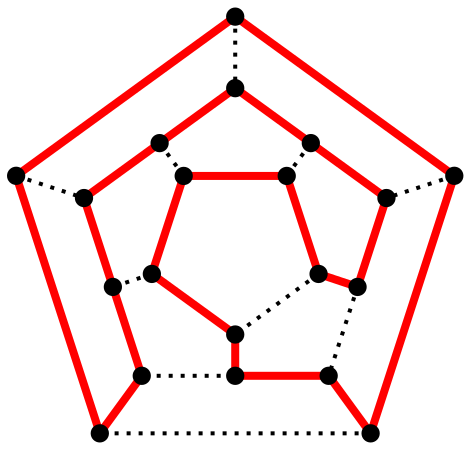
\includegraphics[scale=0.3]{graphs/hamiltonian.png}
  \caption{The red path is a polynomial certificate for the Hamiltonian cycle problem. Source:
  Wikipedia.}
\end{figure}

\begin{definition} The NP class is the set of all decision problems that admit a polynomial
  verifier for the YES answer.
\end{definition}

\begin{definition} The co-NP class is the set of all decision problems that admit a
  polynomial verifier for the NO answer.
\end{definition}

Note how every problem in P is already in NP and co-NP, since the algorithm that solves the problem
could be used as a verifier for both the YES and NO answer.

Let $\Pi$ and $\Pi'$ be problems. A polynomial-time reduction from $\Pi$ to $\Pi'$ is an algorithm
that solves $\Pi$ using an algorithm that solves $\Pi'$ as a subroutine, and that, excluding its
subroutine, is polynomial on the size of its instance. We denote such a reduction by
$\Pi\leq_p\Pi'$ if there exists a polynomial reduction, from $\Pi$ to $\Pi'$.

\begin{algorithm}[h]
  \caption*{\textbf{Problem:} SAT}
  \begin{algorithmic}[1]
    \Require\, A Boolean formula with $n$ variables written in CNF, e.g.\ $(x_1\vee x_2\vee x_2\vee
    x_3)\wedge (\ov{x}_2\vee x_5)\wedge\cdots$
    \Ensure\, Boolean value
    \Description\, Is there a valuation $\nu :\{x_1,x_2,\ldots,x_n\}\to\{\false, \true\}$ such that the
    input formula evaluates to true?
  \end{algorithmic}
\end{algorithm}

\begin{algorithm}[h]
  \caption*{\textbf{Problem:} 3-SAT}
  \begin{algorithmic}[1]
    \Require\, A Boolean formula with $n$ variables written in CNF with at most 3 literals in each
    clause, e.g.\ $(x_1\vee x_2\vee x_3)\wedge(\ov{x}_2\vee\ov{x}_1\vee x_5) \wedge\cdots$
    \Ensure\, Boolean value
    \Description\, Is there a valuation $\nu :\{x_1,x_2,\ldots,x_n\}\to\{\false, \true\}$ such that the
    input formula evaluates to true?
  \end{algorithmic}
\end{algorithm}

We can prove that SAT $\leq_p$ 3-SAT by turning the clauses in the SAT problem into 3-SAT
clauses~\cite{karp}. Recall Karp's 23 NP-complete list of problems. Each nesting means that the
nested item $\Pi'$ and its parent item $\Pi$ obey $\Pi\leq_p\Pi'$. The SAT problem, can also be
reduced to the Hamiltonian cycle problem by turning edges and vertices into SAT clauses. The vertex
cover problem can also be reduced to the Hamiltonian cycle problem~\cite{karp}.

\begin{definition} A problem $\Pi$ in NP is NP-complete if $\forall$ $\Pi' \in \np$,
  $\Pi'\leq_p\Pi$.
\end{definition}

From the Cook-Levin Theorem~\cite{cook,levin}, we know that the SAT problem is NP-complete. So if
$\Pi\leq_p\Pi'$, and $\Pi$ is NP-complete, then $\Pi'$ is also NP-complete. So showing that a
problem $\Pi'$ is NP-complete consists of the following steps:

\begin{enumerate}
  \item Take $\Pi'\in \np$,
  \item Take $\Pi$ NP-complete,
  \item Show that $\Pi\leq_p\Pi'$.
\end{enumerate}

\begin{definition} A problem $\Pi$ is NP-hard if the existence of a polynomial algorithm for $\Pi$
  implies on $\p=\np$.
\end{definition}

So every NP-complete problem is NP-hard, but an NP-hard problem is not necessarily in NP\@.

We wish to show that the 3-SAT problem can be reduced to the quadratic congruence problem, proving
that QCP is NP-complete.

\section{The Reduction}

In this section we first define the Quadratic Congruence Problem (QCP), state the second theorem
in~\cite{qcp1}, quote the algorithm used in the article that will be used in the proof, and then we
show a complete and detailed proof of the reduction.

We first define the QCP as a decision problem.

\begin{algorithm}[h]
  \caption*{\textbf{Problem:} quadratic congruence}
  \begin{algorithmic}[1]
    \Require\, $\alpha,\beta,\gamma\in\mathbb{Z}$
    \Ensure\, Boolean value
    \Description\, Is there a solution $x\in\mathbb{Z}$ where
    \begin{equation*}
      x^2 \equiv\alpha\mod\beta
    \end{equation*}
    and such that $0\leq x\leq\gamma$?
  \end{algorithmic}
\end{algorithm}

It turns out that the QCP is NP-complete, as we shall prove later. One might think that the QCP's
complexity difficulty lies on the factorization of $\beta$. However, even when the full
factorization of $\beta$ is given, as the reduction shows, it is still NP-complete.

Another interesting note regarding the QCP problem is that, finding a solution $x$ without the
second restriction (i.e.\ no upper bound on $x$, $\gamma=\infty$) is solvable in polynomial time if
we are given $\beta$'s factorization. Furthermore, if we assume the Extended Riemann Hypothesis to
be true, the problem is also solvable in polynomial time when $\beta$ is
prime~\cite{garey-johnson}. Additionally, the problem is trivially solvable in pseudo-polynomial
time, meaning given a nondeterministic Turing machine, one can solve by running a ``guess a
solution and check whether it is a correct'' algorithm in polynomial time~\cite{qcp2}.

We now state the theorem that covers the reduction.

\begin{theorem}[Adleman and Manders, 1976]\label{qcp-thm}
  The (problem of accepting the) set of quadratic congruences (in a standard encoding)
  \begin{equation*}
    x^2\equiv\alpha\mod\beta
  \end{equation*}
  with solutions $x\in\omega$ satisfying
  \begin{equation*}
    0\leq x\leq\gamma;\quad \alpha,\beta,\gamma\in\omega
  \end{equation*}
  is NP-complete.
\end{theorem}

It is easy to prove QCP's membership in NP\@. One could design an algorithm that first checks
whether the input instance $x$ obeys the condition $0\leq x\leq\gamma$. If it passes, we simply
check whether $x^2\equiv\alpha\mod\beta$. This algorithm runs in $\bigo(1)$, and thus is
polynomial. This is a polynomial verifier for the YES answer for the QCP, so QCP is in NP\@.

Before we prove~\autoref{qcp-thm}, we first quote the algorithm used in the reduction
from~\cite{qcp2}. We use this algorithm in the proof extensively. In the article, Adleman and
Manders recommend the reader to simply skim over the algorithm, and then to refer it back when
reading the proof. We also recommend this, as the intent of the algorithm is not clear at first
glance.

The algorithm itself is directly quoted from~\cite{qcp2}, but is also used in~\cite{qcp1}. The
former is a modified version of the latter. We chose the first to quote as it looked to be simpler
and cleaner. Comments of the form [Comment: $\ldots$ ] are comments taken directly from the
article.

\subsection{The algorithm}

On input $\phi$, read $\phi$ and eliminate all duplicate conjuncts and those in which, for some
variable $x_i$, both $x_i$ and $\ov{x}_i$ occur. Count the $l$ variables occurring in the remaining
formula $\phi_R$. Let

\begin{equation*}
  \Sigma = \{\sigma_1,\ldots,\sigma_m\}
\end{equation*}

be a standard enumeration of all possible disjunctive clauses, formed from $x_1,\ldots,x_l$ and
their complements, with at most three literals per clause and no variable occurring twice or both
complemented and uncomplemented in a clause. Compute

\begin{equation*}
  \tau_\phi = -\sum_{\sigma_l\in\phi_R}8^j,
\end{equation*}

where, as below, we use $\in$ to denote the relation of an expressing \textit{occurring} in another
expression. [Comment: $\tau_\phi$ is the only quantity computed which depends specifically on
$\phi_R$, rather than just on the number $l$ of variables occurring in $\phi_R$.] Compute:

\begin{align*}
  &f_i^+ = \sum_{x_i\in\sigma_j}8^j, &i=1,2,\ldots,l,\\
  &f_i^- = \sum_{\ov{x}_i\in\sigma_j}8^j, &i=1,2,\ldots,l.
\end{align*}

Set $n=2m+l$ and compute $c_j,j=0,\ldots,n$, as

\begin{align*}
  &\;c_0=1\\
  &\begin{rcases*}
  c_j=-\frac{1}{2}8^k,\qquad &j=2k-1,\\
  c_j=-8^k,\qquad &j=2k,\\
  \end{rcases*} &j=1,\ldots,2m\\
  &\;c_{2m+j}=\frac{1}{2}(f_j^+ - f_j^-), &j=1,2,\ldots,l,
\end{align*}

and

\begin{equation*}
  \tau = \tau_\phi + \sum_{j=0}^n c_j + \sum_{i=1}^l f_i^-
\end{equation*}

[Comment: At this point we have in fact obtained a knapsack problem $sum_{j=0}^n c_j\alpha_j=\tau$,
$\alpha_j\in\{-1, +1\}$, which is solvable if and only if $\phi$ is satisfiable; moreover, for any
value of $\alpha_j\in\{-1,+1\}$, $|\sum_{j=0}^n c_j\alpha_j -\tau|<8^{m+1}$, so the knapsack
problem is equivalent to $\sum_{j=0}^n c_j\alpha_j\equiv\tau\mod 8^{m+1}$, $\alpha_j\in\{-1,+1\}$.
These assertions will become clear from the proof of correctness.]

Determine the first $n+1$ primes, $p_0,\ldots,p_n$, exceeding

\begin{equation*}
  {(4(n+1)8^{m+1})}^\frac{1}{n-1}
\end{equation*}

[This is in fact never exceeds 12, so we can set $p_0=13$.]

Determine parameters $\theta_j$, $j=0,1,\ldots,n$, as: the least $\theta_j\in\omega$ such that

\begin{flalign*}
  &\theta_j\equiv c_j\mod 8^{m+1},\\
  &\theta_j\equiv 0\mod \prod_{i\neq j}^n p_i^{n+1},\\
  &\theta_j\not\equiv 0\mod p_j.
\end{flalign*}

(Note: the following part of the algorithm was changed since Theorem 1 in article~\cite{qcp2} is
the quadratic Diophantine solutions problem and Theorem 2 is the QCP\@. In our paper, we refer to
Theorem 1 as the QCP, and Theorem 2 as the Diophantine problem.)

Compute $H=\sum_{j=0}^n \theta_j$, $K=\prod_{j=0}^n p_j^{n+1}$ and output:

\begin{enumerate}[label= (\alph*)]
  \item for Theorem 1 (QCP):

    \begin{align*}
      x^2\equiv {(2\cdot 8^{m+1}+K)}^{-1}\cdot(K\tau^2+2\cdot 8^{m+1}H^2)\mod 2\cdot 8^{m+1}\cdot
        K,\quad 0\leq x\leq H,\\
      \text{where, } {(2\cdot 8^{m+1}+K)}^{-1}\text{ is the inverse of }(2\cdot 8^{m+1}+K)\mod
      2\cdot 8^{m+1} \cdot K^n.\\
    \end{align*}

  \item for Theorem 2 (Diophantine):

    \begin{align*}
      {(K+1)}^3\cdot 2\cdot 8^{m+1}\cdot(H^2-x_1^2)+K(x_1^2-\tau^2)-x_2\cdot 2\cdot 8^{m+1}\cdot K=0.
    \end{align*}
\end{enumerate}

\subsection{The proof}

In this subsection we show the proof of correctness of the algorithm (i.e.\ the proof of the
reduction). We follow the proof given in~\cite{qcp2}, but with all passages explicitly explained,
as well as a proof of Lemma 2 that was left to the reader.

We need to first show that the propositional formula $\phi$ is satisfiable if and only if the
following expression is solvable.

\begin{equation*}
  \sum_{j=0}^n \theta_j\alpha_j\equiv\tau\mod 8^{m+1},\qquad\alpha_j\in\{-1,+1\},\quad j=0,\ldots,n
\end{equation*}

It is easy to see that the formula $\phi_R$ is satisfiable if and only if $\phi$ is, since $\phi_R$
is the result of taking out all irrelevant clauses. But $\phi_R$ is satisfiable if and only if
there is a valuation $r:\{x_1,\ldots,x_l\}\to\{0,1\}$ such that for each disjunctive clause
$\sigma_k\in\Sigma$

\begin{equation}\label{eq-rk}
  0 = R_k
  \begin{dcases}
    =y_k-\sum_{x_i\in\sigma_k} r(x_i)-\sum_{\ov{x}_i\in\sigma_k} (1-r(x_i))+1, \quad&\text{if }
    \sigma_k\in\phi_R,\hfill(1)\\
    =y_k-\sum_{x_i\in\sigma_k} r(x_i)-\sum_{\ov{x}_i\in\sigma_k} (1-r(x_i)), \quad&\text{if }
    \sigma_k\not\in\phi_R.\hfill(2)
  \end{dcases}
\end{equation}

is solvable by $y_k\in\{0,1,2,3\}$. We also add the constraint

\begin{equation*}
  0 = R_0 = \alpha_0 + 1, \qquad \alpha_0\in\{0, 1\}
\end{equation*}

that does not influence the satisfiability of the system. We next prove that~\autoref{eq-rk} does
in fact hold for the if and only if satisfiability.

\begin{proof}[Proof of \autoref{eq-rk}]
  We first consider case (1):

  \begin{equation*}
    0 = y_k-\sum_{x_i\in\sigma_k} r(x_i)-\sum_{\ov{x}_i\in\sigma_k} (1-r(x_i))+1,\quad\text{if }
    \sigma_k\in\phi_R
  \end{equation*}

  So $y_k$ must be of the form:

  \begin{equation*}
    y_k=\sum_{x_i\in\sigma_k} r(x_i)+\sum_{\ov{x}_i\in\sigma_k} (1-r(x_i))-1
  \end{equation*}

  With no loss of generality, we can enumerate all possible clauses $\sigma_k$ as follows

  \begin{align*}
    &(x_p\vee x_q\vee x_t): &y_k=r(x_p)+r(x_q)+r(x_t)-1\implies &-1\leq y_k\leq 2\\
    &(\ov{x}_p\vee x_q\vee x_t): &y_k=r(x_q)+r(x_t)+1-r(x_p)-1\implies &-1\leq y_k\leq 2\\
    &(\ov{x}_p\vee\ov{x}_q\vee x_t):&y_k=r(x_t)+2-r(x_p)-r(x_q)-1\implies &-1\leq y_k\leq 2\\
    &(\ov{x}_p\vee\ov{x}_q\vee\ov{x}_t):&y_k=3-r(x_p)-r(x_q)-r(x_t)-1\implies &-1\leq y_k\leq 2
  \end{align*}

  Note how in all cases above, the clause is satisfiable if and only if $y_k\neq -1$. In the first
  case, when $y_k=-1$, no literal $x_i$ is valuated as true. In the second case, when $y_k\neq -1$,
  no literal $x_i$ is valuated as true and $\ov{x}_p$ is valuated as false. The third case is
  similar, with $x_t$ false, and $\ov{x}_p,\ov{x}_q$ false. For the last case, all $\ov{x}_i$ are
  set to false. When $y_k\neq -1$, there exists some literal being valuated as true, and therefore
  the clause $\sigma_k$ is valuated as true.

  For case (2), we do the same. In this case, $y_k$ is of the form:

  \begin{equation*}
    y_k=\sum_{x_i\in\sigma_k} r(x_i)+\sum_{\ov{x}_i\in\sigma_k} (1-r(x_i))
  \end{equation*}

  Enumerating all literal combinations we have:

  \begin{align*}
    &(x_p\vee x_q\vee x_t): &y_k=r(x_p)+r(x_q)+r(x_t)\implies &0\leq y_k\leq 3\\
    &(\ov{x}_p\vee x_q\vee x_t): &y_k=r(x_q)+r(x_t)+1-r(x_p)\implies &0\leq y_k\leq 3\\
    &(\ov{x}_p\vee\ov{x}_q\vee x_t):&y_k=r(x_t)+2-r(x_p)-r(x_q)\implies &0\leq y_k\leq 3\\
    &(\ov{x}_p\vee\ov{x}_q\vee\ov{x}_t):&y_k=3-r(x_p)-r(x_q)-r(x_t)\implies &0\leq y_k\leq 3
  \end{align*}

  The analysis for this case goes analogally to the previous case, but with $y_k=0$ being
  instatisfiable. Note how $y_k=0$ is still a solution to the previous case. This inconsistency
  does not break the hypothesis, since in (2) we are considering clauses $\sigma_k\not\in\phi_R$.
  That is, $\sigma_k$ does not need to necessarily satisfy for $\phi_R$ to satisfy. However, for
  $\phi_R$ to be satisfiable, $y_k$ needs to be in $\{0,1,2,3\}$, as we showed.
\end{proof}

In order for $\phi_R$ to be satisfiable, every $\sigma_k\in\phi_R$ must be satisfiable. This is an
if and only if condition on $y_k\in\{0,1,2,3\}$, as we showed earlier. For any satisfiable
$\phi_R$, we have the following inequalities.

\begin{align*}
  -3&\leq R_k\leq 4, \quad &k=1,2,\ldots,m\\
  0&\leq R_0\leq 2
\end{align*}

From this, it follows that

\begin{equation}\label{eq-1}
  R_k=0, \quad k=0,1,\ldots,m \iff \sum_{k=0}^m R_k\cdot 8^k = 0
\end{equation}

and also that

\begin{equation}\label{eq-2}
  \left| \sum_{k=0}^m R_k\cdot 8^k \right| < 8^{m+1}
\end{equation}

This is true because

\begin{align*}
  \left|\sum_{k=0}^m R_k\cdot 8^k\right|=\left|R_0\cdot 8^0+\sum_{k=1}^m R_k\cdot 8^k\right|&\leq
    2+\sum_{k=1}^m 4\cdot 8^k\\
    &\leq 2+(4\cdot 8+4\cdot 8^2+\cdots+4\cdot 8^m)\\
    &\leq2+8\underbrace{(4+4\cdot 8+4\cdot 8^2+\cdots+4\cdot 8^{m-1})}_{\text{geometric series}}\\
    &\leq 2+ 8\left(\frac{4}{7}\cdot 8^m-\frac{4}{7}\right)\\
    &\leq 2+\frac{4}{7}\cdot 8^{m+1} -8\cdot\frac{4}{7}\\
    &< 8^{m+1}
\end{align*}

From (\ref{eq-1}) and (\ref{eq-2}), we have that

\begin{equation}\label{eq-3}
  R_k=0,\quad k=0,1,\ldots,m \iff \sum_{k=0}^m R_k\cdot 8^k\equiv 0\mod 8^{m+1}.
\end{equation}

We now wish to prove that we can reorganize the RHS of~\autoref{eq-3} into the following expression
by using the terms from the algorithm. That is, that

\begin{equation}\label{eq-p2}
 \sum_{k=0}^m R_k\cdot 8^k\equiv 0\mod 8^{m+1}\iff\sum_{j=0}^n c_j\alpha_j\equiv\tau\mod 8^{m+1}.
\end{equation}

\begin{proof}[Proof of \autoref{eq-p2}]

We replace variables $y_k$ and valuations $r(x_i)$ by $\{-1,+1\}$-valued variables:

\begin{align*}
  y_k=&\frac{1}{2}\left[\left(1-\alpha_{2k-1}\right)+2\cdot\left(1-\alpha_{2k}\right)\right]\\
  r(x_i)=&\frac{1}{2}\left(1-\alpha_{2m+i}\right)
\end{align*}

We call $R_k'$ the result of this substitution. It follows that

\begin{equation*}
  R_k'=\frac{1}{2}[(1-\alpha_{2k-1})+2(1-\alpha_{2k})]-\sum_{x_i\in\sigma_k}\frac{1}{2}(1-
  \alpha_{2m+i})-\sum_{\ov{x}_i\in\sigma_k}\left[1-\frac{1}{2}(1-\alpha_{2m+i})\right]+1
\end{equation*}

when $\sigma_k\in\phi_R$. Plugging $R_k'$ into (\ref{eq-3}) gives us

\begin{equation}\label{eq-4}
  \sum_{k=0}^m\left(\frac{8^k}{2}-\frac{8^k}{2}\alpha_{2k-1}+8^k-8^k\alpha_{2k}-
  \sum_{x_i\in\sigma_k}\left(\frac{8^k}{2}-\frac{8^k}{2}\alpha_{2m+i}\right)-
  \sum_{\ov{x}_i\in\sigma_k}\left(\frac{8^k}{2}+\frac{8^k}{2}\alpha_{2m+i}\right)+8^k\right)\equiv
  0\mod 8^{m+1}
\end{equation}

Recall the $c_j$, $j=0,1,\ldots,n$ variables computed earlier in the algorithm:

\begin{align*}
  &\begin{rcases*}
    c_{2k-1}=-\frac{1}{2}8^k\\
    c_{2k}=-8^k\\
  \end{rcases*} &j=1,\ldots,2m\\
  &\;c_{2m+j}=\frac{1}{2}(f_j^+-f_j^-), &j=1,2,\ldots,l
\end{align*}

We wish to take equation (\ref{eq-4}) and make it look like

\begin{equation*}
  \sum_{j=0}^n c_j\alpha_j\equiv\tau\mod 8^{m+1}, \quad\alpha_j\in\{-1,+1\}.
\end{equation*}

Replacing the values from (\ref{eq-4}) with the corresponding $c_j$ values gives us

\begin{equation}\label{eq-5}
  \sum_{k=0}^m\left(\underbrace{-c_{2k-1}+c_{2k-1}\alpha_{2k-1}-c_{2k}+c_{2k}\alpha_{2k}}_{(\star)}
  -\underbrace{\sum_{x_i\in\sigma_k}8^k\left(\frac{1}{2}-\frac{1}{2}\alpha_{2m+i}\right)-\sum_{
  \ov{x}_i\in\sigma_k}8^k\left(\frac{1}{2}+\frac{1}{2}\alpha_{2m+i}\right)}_{(\star\star)}+
  \underbrace{8^k}_{(\star\star\star)}\right)
\end{equation}

on the LHS\@. We first turn our attention to $(\star)$. Notice how the pair $(2k-1,2k)$ over the
range $[0,m]$ covers the range $[0,2m]$, meaning that

\begin{equation*}
  \sum_{k=0}^m \left(c_{2k-1}+c_{2k}\right) = \sum_{i=0}^{2m} c_{i}.
\end{equation*}

In particular, separating the terms of the summation into two parts gives us

\begin{equation*}
  \overbrace{\sum_{k=0}^m\left(c_{2k-1}\alpha_{2k-1}\right)-\sum_{k=0}^m\left(c_{2k-1}+c_{2k}
  \right)}^{(\star)} = \sum_{j=0}^{2m}c_j\alpha_j-\sum_{j=0}^{2m}c_j
\end{equation*}

Recall from the algorithm that

\begin{align*}
  &f_i^+ = \sum_{x_i\in\sigma_j}8^j, &i=1,2,\ldots,l,\\
  &f_i^- = \sum_{\ov{x}_i\in\sigma_j}8^j, &i=1,2,\ldots,l.
\end{align*}

Since $f_j^+$ and $f_j^-$ are both counting the number of literals in $\phi_R$, it is easy to see
that $\sum_{x_i\in\phi_R}f_i^+=\sum_{\ov{x}_i\in\phi_R}f_i^-$, since they range over all
$\sigma_k$, and $\Sigma$ is the set of all $\sigma_k$ relevant clause permutations. So every
literal $x_i$ must appear the same number of times as $\ov{x}_i$. This means $\sum_{j=1}^l c_{2m+j}
= 0$. Note how there exactly $l$ variables in $\phi_R$. From this we have that

\begin{equation*}
  \sum_{j=0}^{2m}c_j\alpha_j-\sum_{j=0}^{2m}c_j = \sum_{j=0}^n c_j\alpha_j-\sum_{j=0}^n c_j.
\end{equation*}

We now consider $(\star\star)$. It follows from $(\star\star)$ that

\begin{equation*}
  -\underbrace{\sum_{x_i\in\sigma_k}\frac{8^k}{2}}_{\frac{f_i^+}{2}}-
  \underbrace{\sum_{\ov{x}_i\in\sigma_k}\frac{8^k}{2}}_{\frac{f_i^-}{2}}-\frac{8^k}{2}
  \underbrace{\left(\sum_{x_i\in\sigma_k}\alpha_{2m+i}-\sum_{\ov{x}_i\in\sigma_k}\alpha_{2m+i}
  \right)}_{=0\text{ when summing over $[0,m]$}} = -\sum_{\hat{x}_i\in\sigma_k}
  \frac{1}{2}\left(f_i^++f_i^-\right)
\end{equation*}

where we say $\hat{x}_i\in\sigma_k$ if $x_i\in\sigma_k$ or $\ov{x}_i\in\sigma_k$. The same argument
from $(\star)$ can be used to show that

\begin{equation*}
  -\sum_{k=0}^m\sum_{\hat{x}_i\in\sigma_k}\frac{1}{2}(f_i^++f_i^-)=-\sum_{k=0}^m\sum_{\hat{x}_i
  \in\sigma_k}f_i^-
\end{equation*}

Now we have a summation over all disjunctive clauses $\sigma_k$, and for each $k$ we are summing
all occurrences in which $\hat{x}_i\in\sigma_k$. But this means we are summing all times in which
each variable occurs in all clauses. The number of variables is $l$, so it follows that

\begin{equation*}
  -\sum_{k=0}^m\sum_{\hat{x}_i\in\sigma_k}f_i^- =-\sum_{i=1}^l f_i^-.
\end{equation*}

Let us now focus on $(\star\star\star)$. It is easy to see that

\begin{equation*}
  \sum_{k=0}^m 8^k = \sum_{\sigma_j\in\phi_R} 8^j = -\tau_\phi
\end{equation*}

Plugging the results (note that these results already take into account the outer summation
$\sum_{k=0}^m$, and thus we ommit it) from $(\star), (\star\star), (\star\star\star)$ in
\autoref{eq-5} gives us the following expression:

\begin{equation*}
  \underbrace{\sum_{j=0}^n c_j\alpha_j-\sum_{j=0}^n c_j}_{(\star)}-\underbrace{\sum_{i=1}^l
  f_i^-}_{(\star\star)}-\underbrace{\tau_\phi}_{(\star\star\star)}\equiv 0\mod 8^{m+1}
\end{equation*}

Isolating the first summation of $(\star)$ yields

\begin{equation*}
  \sum_{j=0}^n c_j\alpha_j\equiv\tau_\phi+\sum_{j=0}^n c_j+\sum_{i=1}^l f_i^-\mod 8^{m+1}
\end{equation*}

The RHS of the congruence is exactly the definition of $\tau$ from the algorithm. Therefore:

\begin{equation*}
  \sum_{j=0}^n c_j\alpha_j\equiv\tau\mod 8^{m+1}, \quad\alpha_j\in\{-1,+1\}
\end{equation*}

\end{proof}

From the definition of $\theta_j$, $j=0,\ldots,n$, it follows directly that the above is equivalent
to

\begin{equation*}
  \sum_{j=0}^n\theta_j\alpha_j\equiv\tau\mod 8^{m+1}, \quad\alpha_j\in\{-1,+1\}
\end{equation*}

\begin{lemma}\label{lemma-1}
  Let $K$ and $H$ be as in the algorithm. The general solution of the system
  \begin{align*}
    &0\leq|x|\leq H, \qquad x\in\mathbb{Z} \quad &(1)\\
    &(H+x)(H-x)\equiv 0\mod K &(2)
  \end{align*}
  is given by
  \begin{equation*}
    x=\sum_{j=0}^n\alpha_j\theta_j, \quad\alpha_j\in\{-1,+1\},\quad j=0,1,\ldots,n.
  \end{equation*}
\end{lemma}
\begin{proof}
  Let us recall the definitions of $K$ and $H$ from the algorithm:

  \begin{align*}
    &K=\prod_{i=0}^n p_i^{n+1} \quad\text{, where $p_0=13$ and $p_1,p_2,\ldots,p_n$ primes
    exceeding 12.}\\
    &H=\sum_{i=0}^n\theta_i
  \end{align*}

  It is obvious that $x$ is a solution to the system. We need to prove that these are the only
  solutions to the system. Let $x$ be a solution to the system. Then

  \begin{equation*}
    (H+x)(H-x)\equiv 0\mod p_j^{n+1}, \qquad j=0,1,\ldots,n
  \end{equation*}

  We will prove by contradiction. Assume that for some $j_0$:

  \begin{equation*}
    p_{j_0}|(H+x)\text{ and }p_{j_0}|(H-x)
  \end{equation*}

  Then $p_{j_0}|(H+x)+(H-x)=2H$. But $p_{j_0}>2$ and $p_{j_0}$ is prime, so $p_{j_0}|H$. It then
  follows that $p_{j_0}|\sum_{j=0}^n\theta_j$. But from the definition of $\theta_j$, we know that
  $p_{j_0}|\theta_j$ for all $j\neq j_0$, since we have

  \begin{equation*}
    \theta_j\equiv 0\mod\prod_{i\neq j}^n p_i^{n+1}\implies\prod_{i\neq j}^n p_i^{n+1}|\theta_j
    \implies p_i|\theta_j, \quad i\neq j
  \end{equation*}

  So it must be that $p_{j_0}|\theta_{j_0}$, but from $\theta_j$'s definition:

  \begin{equation*}
    \theta_j\not\equiv 0\mod p_j\implies p_j\nmid\theta_j
  \end{equation*}

  We end up in a contradiction. Therefore we can conclude that for all $j$, $p_j^{n+1}$ divides
  either $(H+x)$ or $(H-x)$, but not both.

  We define:

  \begin{align*}
    &\alpha_j=
    \begin{cases}
      \phantom{-}1,  &\quad \text{if } p_j^{n+1}|(H-x)\\
      -1,  &\quad \text{if } p_j^{n+1}|(H+x)
    \end{cases}\\
    &x'=\sum_{j=0}^n\alpha_j\theta_j
  \end{align*}

  So we have $x'\equiv\alpha_j\theta_j\equiv\alpha_j H\equiv x\mod p_j^{n+1}$, and $x'\equiv x\mod
  p_j^{n+1}$, for all $j$, and so $x'\equiv x\mod K$.

  \begin{equation*}
    \begin{rcases}
      & -H\leq x'\leq H\\
      & -H\leq x\leq H\\
    \end{rcases} \implies |x-x'|\leq 2H
  \end{equation*}

  But $p_j\geq{(4(n+1)8^{m+1})}^\frac{1}{n+1}$, and let

  \begin{equation*}
    \lambda_j=\frac{\theta_j}{\sum_{\substack{i=0\\i\neq j}}^n p_i^{n+1}}
  \end{equation*}

  We have that $\lambda_j<2\cdot 8^{m+1}$ for each $j$. Each term in $H$ is bounded by $K/2(n+1)$,
  so $2H<K$. This means $|x-x'|<K$, but $x'\equiv x\mod K$. Therefore, it must be that $x=x'$.

  Thus $x'$ is a solution and is the same as $x$, meaning any solution of the system is of that
  form.
\end{proof}

From~\autoref{lemma-1}, the condition

\begin{equation*}
  \sum_{j=0}^n\theta_j\alpha_j\equiv\tau\mod 8^{m+1}
\end{equation*}

is equivalent to the system:

\begin{align*}
  (i) \quad &0\leq|x|\leq H, \quad x\in\mathbb{Z},\\
  (ii) \quad &x\equiv\tau\mod 8^{m+1}, &\text{(I)}\\
  (iii) \quad &(H+x)(H-x)\equiv 0\mod K
\end{align*}

\begin{lemma}\label{lemma-2}
  Let $\tau$ be odd, $x\in\mathbb{Z}$, $k\geq 3$
  \begin{align*}
    (\tau+x)(\tau-x)\equiv 0\mod 2^{k+1}\iff\text{ either }\;&\tau+x\equiv 0\mod 2^k\\
                                            \text{ or }\;&\tau-x\equiv 0\mod 2^k
  \end{align*}
\end{lemma}
\begin{proof}
  We first prove the converse $(\impliedby)$:

  Assume it is possible for both cases to be true.
  \begin{align*}
    &\tau+x\equiv 0\mod 2^k\implies\tau\equiv -x\mod 2^k\\
    &\tau-x\equiv 0\mod 2^k\implies\tau\equiv \phantom{-}x\mod 2^k
  \end{align*}
  So $\tau\equiv x\equiv 0\mod 2^k$. But $\tau$ is odd, leading to a contradiction. Therefore, only
  one of the two can be true at the same time. Consider the first case ($\tau+x\equiv 0\mod 2^k$).
  So $(\tau+x)\equiv 0\mod 2^k\implies(\tau+x)(\tau-x)\equiv 0\mod 2^k$. In other words,
  $(\tau+x)(\tau-x)= 2^k \cdot c$. Multiplying $2$ on both sides yields $2(\tau+x)(\tau-x)
  =2^{k+1}\cdot c$. Converting it back to its congruence form gives us $2(\tau+x)(\tau-x)\equiv
  0\mod 2^{k+1}$. But $\tau+x\equiv 0\mod 2^k$, so we can substitute $(\tau+x)$ for $2^k$, giving
  $2\cdot 2^k\cdot c(\tau-x)=2^{k+1}c(\tau-x)\equiv 0\mod 2^{k+ 1}$.  We do the same for
  $\tau-x\equiv 0\mod 2^k$.

  We now prove the direct implication $(\implies)$:

  \begin{align*}
    (\tau+x)(\tau-x)\equiv 0\mod 2^{k+1}\implies\text{ either }\;&\tau+x\equiv 0\mod 2^k\\
                                            \text{ or }\;&\tau-x\equiv 0\mod 2^k
  \end{align*}

  We can rewrite $(\tau+x)(\tau-x)\equiv 0\mod 2^{k+1}$ as $(\tau+x)(\tau-x)=2^{k+1}\cdot c=2^k(2c)
  =(\tau+x)(\tau-x)$. So $(\tau+x)(\tau-x)\equiv 0\mod 2^k$.

  Let $a=\tau+x$ and $b=\tau-x$. We need to show that the cases:
  \begin{align*}
    (1) \quad &a\equiv 0\mod 2^k\quad\text{and}\quad b\neq 0\mod 2^k\\
    (2) \quad &b\not\equiv 0\mod 2^k\quad\text{and}\quad b\not\equiv 0\mod 2^k
  \end{align*}
  are impossible if $a\cdot b\equiv 0\mod 2^k$. We take case (1) into consideration first.

  \begin{equation*}
    \begin{cases}
      &\tau+x\equiv 0\mod 2^k\\
      &\tau-x\equiv 0\mod 2^k\\
    \end{cases}
  \end{equation*}

  But from the converse's proof, we know that this is impossible. Now we consider the second case.

  \begin{align*}
    \begin{cases}
      &\tau+x\not\equiv 0\mod 2^k\\
      &\tau-x\not\equiv 0\mod 2^k\\
      &(\tau+x)(\tau-x)\equiv 0\mod 2^k\\
    \end{cases}\quad&\implies&
    \begin{cases}
      &2^k\nmid\tau+x\\
      &2^k\nmid\tau-x\\
      &2^k\nmid(\tau+x)(\tau-x)\\
    \end{cases}
  \end{align*}

  Which is a contradiction. Therefore, the two cases are impossible. It is easy to see that all the
  remaining cases are the ones listed in the Lemma, and all are true.
\end{proof}

Consider the system (I). The conditions of~\autoref{lemma-2} apply to the system. Therefore system
(I) is satisfiable if and only if system (II) is also satisfiable:

\begin{align*}
  (i) \quad &0\leq|x|\leq H, \quad x\in\mathbb{Z},\\
  (ii) \quad &(\tau+x)(\tau-x)\equiv 0\mod 2\cdot 8^{m+1}, &\text{(II)}\\
  (iii) \quad &(H+x)(H-x)\equiv 0\mod K
\end{align*}

From~\autoref{lemma-2}, (I)\,(ii) satisfies if and only if (II)\,(iii) satisfies, since if $\tau-x
\equiv 0\mod 8^{m+1}$, then it satisfies (I)\,(ii); and if $\tau+x\equiv 0\mod 8^{m+1}$, then it
satisfies (i) and (iii).

Note how:

\begin{align*}
  (i) \quad &(\tau+x)(\tau-x)\equiv\tau^2-x^2\equiv 0\mod 2\cdot 8^{m+1}\\
  (ii) \quad &(H+x)(H-x)\equiv H^2-x^2\equiv 0\mod K
\end{align*}

So we can restrict condition (i) to only positive integers:

\begin{equation*}
  0\leq x_1\leq H, \quad x_1\in\mathbb{Z}
\end{equation*}

Also note that $\gcd(2\cdot 8^{m+1}, K)=1$, since $K$ is a product of odd primes (in fact greater
than 12) and $2\cdot 8^{m+1}$ a power of 2. Because of that, we can join both conditions (ii) and
(iii) from system (II).

\begin{equation*}
  \lambda_1 2\cdot 8^{m+1}(H^2-x_1^2)+\lambda_2 K(\tau^2-x_1^2)\equiv 0\mod 2\cdot 8^{m+1}\cdot K
\end{equation*}

Where $\lambda_1$ and $\lambda_2$ are parameters we can freely choose subject to the following
condition:

\begin{equation*}
  \gcd(\lambda_1,K)=\gcd(\lambda_2,2\cdot 8^{m+1})=1,\quad\lambda_1,\lambda_2\in\mathbb{Z}
\end{equation*}

We join these conditions into the new system (III):

\begin{align*}
  (i) \quad &0\leq x_1\leq H, \quad x_1\in\mathbb{Z},\\
  (ii) \quad &\lambda_1 2\cdot 8^{m+1}(H^2-x_1^2)+\lambda_2 K(\tau^2-x_1^2)\equiv 0\mod 2\cdot
    8^{m+1}\cdot K, &\text{(III)}\\
  (iii) \quad &\gcd(\lambda_1,K)=\gcd(\lambda_2,2\cdot 8^{m+1})=1,\quad\lambda_1,\lambda_2\in
    \mathbb{Z}.
\end{align*}

In fact, choosing $\lambda_1$ and $\lambda_2$ provides proofs for two problems: the quadratic
Diophantine problem (which we will mention later) and for the QCP\@. Furthermore, conditions
(III)\,(i),\,(ii) are satisfiable for any $\lambda_1,\lambda_2$ obeying (III)\,(iii) or for no
$\lambda_1$ and $\lambda_2$.

We now finally provide a proof for~\autoref{qcp-thm}.

\begin{proof}[Proof of~\autoref{qcp-thm}]
  Choose $\lambda_1=\lambda_2=1$. It obviously satisfies (III)\,(iii). We rewrite (III)\,(ii) with
  these values:
  \begin{align*}
    &2\cdot 8^{m+1}(H^2-x_1^2)+K(\tau^2-x_1^2)\equiv 0\mod 2\cdot 8^{m+1}\cdot K\\
    &2\cdot 8^{m+1}H^2-2\cdot 8^{m+1}x_1^2+K\tau^2-x_1^2K\equiv 0\mod 2\cdot 8^{m+1}\cdot K\\
    &K\tau^2+2\cdot 8^{m+1}\cdot H^2\equiv(2\cdot 8^{m+1}+K)\cdot x_1^2\mod 2\cdot 8^{m+1}\cdot K
  \end{align*}
  Note how $\gcd(2\cdot 8^{m+1}+K,2\cdot 8^{m+1}\cdot K)=1$, and as such there exists an inverse
  ${(2\cdot 8^{m+1}+K)}^{-1}$. Multiplying the inverse on both sides, yields:

  \begin{equation*}
    {(2\cdot 8^{m+1}+K)}^{-1}\cdot(2\cdot 8^{m+1}+K)x_1^2\equiv{(2\cdot 8^{m+1}+K)}^{-1}(K\tau^2+
    2\cdot 8^{m+1}\cdot H^2)\mod 2\cdot 8^{m+1}\cdot K
  \end{equation*}

  Rewriting the expression above gives us:

  \begin{equation*}
    x_1^2\equiv {(2\cdot 8^{m+1}+K)}^{-1}(K\tau^2+2\cdot 8^{m+1}\cdot H^2)\mod 2\cdot 8^{m+1}\cdot K
  \end{equation*}

  Note how this is exactly the output of the algorithm for the QCP\@. Call $\alpha={(2\cdot
  8^{m+1}+K)}^{-1}(K\tau^2+2\cdot 8^{m+1}\cdot H^2)$ and $\beta=2\cdot 8^{m+1}\cdot K$. Rename
  $x_1$ as $x$. Note how we now have:

  \begin{equation*}
    x^2\equiv\alpha\mod\beta
  \end{equation*}

  Renaming $H$ as $\gamma$ gives us the restriction

  \begin{equation*}
    0\leq x^2\leq\gamma
  \end{equation*}

  where $\alpha,\beta,\gamma\in\omega$. But this is exactly the theorem. So the QCP is satisfiable
  if and only if system (III) is satisfiable. But (III) is satisfiable if and only if the
  propositional formula (i.e.\ 3-SAT) is satisfiable. From this we conclude that QCP is
  NP-complete.
\end{proof}

\section{Related problems}

Manders and Adleman proved in both~\cite{qcp1,qcp2} that not only the QCP is NP-complete, but also
the following:

\begin{theorem}\label{diophantine-thm}
  The (problem of accepting the) set of Diophantine equations (in a standard binary encoding) of
  the form
  \begin{equation*}
    \alpha x_1^2+\beta x_2-\gamma=0;\quad\alpha,\beta,\gamma\in\omega,
  \end{equation*}
  which have natural-number solutions $x_1,x_2$ is NP-complete.
\end{theorem}

The proof of this theorem starts exactly as the reduction we showed, with the only difference being
in the choice of $\lambda_1$ and $\lambda_2$. We leave it to the reader to prove this (take
$\lambda_1={(K+1)}^3$ and $\lambda_2=-1$).

\begin{algorithm}[h]
  \caption*{\textbf{Problem:} 0\texttt{-}1 knapsack}
  \begin{algorithmic}[1]
    \Require\, Set of $n$ items, weights $w_1,\ldots,w_n$, values $v_1,\ldots,v_n$ and maximum
    capacity $W$, all positive integers
    \Description\, Can a value of at least $V$ be achieved without exceeding $W$?
    \Reduction\, Exact cover
    \Reference\, [Karp, 1972 (\cite{karp})]
  \end{algorithmic}
\end{algorithm}

When describing the algorithm in~\cite{qcp2}, Adleman and Manders commented on the algorithm's
similarity to the Knapsack problem. In fact, we can reduce QCP to Knapsack, as the algorithm for
Knapsack can be used as a subroutine for the algorithm quoted in this paper. In fact, Knapsack is
satisfiable if and only if $\sum_{j=0}^n c_j\alpha_j\equiv\tau\mod 8^{m+1}$.

We end this paper with a list of selected Number Theory problems that were shown to be NP-complete.
This list was extracted from~\cite{garey-johnson}. All the following problems are decision
problems, meaning we will ommit their output, as they should all return a boolean value.  We label
as \textbf{Reduction} the transformation done in the proof (e.g.\ the 3-SAT was reduced to the QCP
in our proof), and as \textbf{Reference} the article with the reduction. The field \textbf{Comment}
contains comments given by Garey and Johnson on each problem~\cite{garey-johnson}.

\begin{algorithm}[h]
  \caption*{\textbf{Problem:} simultaneous incongruences}
  \begin{algorithmic}[1]
    \Require\, Collection $\{(a_1,b_1),\ldots,(a_n,b_n)\}$ of ordered pairs of positive integers,
    with $a_i\leq b_i$ for $1\leq i\leq n$
    \Description\, Is there an integer $x$ such that, for $1\leq i\leq n, x\not\equiv a_i\mod b_i$?
    \Reduction\, 3-SAT
    \Reference\,~\cite{stockmeyer-meyer}
  \end{algorithmic}
\end{algorithm}

\begin{algorithm}[h]
  \caption*{\textbf{Problem:} root of modulus 1}
  \begin{algorithmic}[1]
    \Require\, Ordered pairs $(a[i],b[i])$, $1\leq i\leq n$, of integers, with each $b[i]\geq 0$.
    \Description\, Does the polynomial $\sum_{i=1}^n a[i]\cdot z^{b[i]}$ have a root on the complex
    unit circle, i.e., is there a complex number $q$ with $|q|=1$ such that $\sum_{i=1}^n a[i]\cdot
    q^{b[i]}=0$?
    \Reduction\, 3-SAT
    \Reference\,~\cite{plaisted-77b}
    \Commentx\, Not known to be in NP or co-NP\@.
  \end{algorithmic}
\end{algorithm}

\begin{algorithm}[h]
  \caption*{\textbf{Problem:} cosine product integration}
  \begin{algorithmic}[1]
    \Require\, Sequence $(a_1,a_2,\ldots,a_n)$ of integers
    \Description\, Does $\int_0^{2\pi}(\prod_{i=1}^n \cos(a_i\theta))d\theta=0$?
    \Reduction\, Partition
    \Reference\,~\cite{plaisted-76}
    \Commentx\, Solvable in pseudo-polynomial time.
  \end{algorithmic}
\end{algorithm}

\begin{algorithm}[h]
  \caption*{\textbf{Problem:} non-trivial greatest common divisor}
  \begin{algorithmic}[1]
    \Require\, Sequences $A_i=<(a_i[1],b_i[1]),\ldots,(a_i[k],b_i[k])>$, $1\leq i\leq m$, of pairs
    of integers, with each $b_i[j]\geq 0$.
    \Description\, Does the $\gcd$ of the polynomials $\sum_{j=1}^k a_i[j]\cdot z^{b_i[j]}$, $1\leq
    i\leq m$, have a degree greater than zero?
    \Reduction\, 3-SAT
    \Reference\,~\cite{plaisted-77a}
    \Commentx\, Not known to be in NP or co-NP\@. Remains NP-hard if each $a_i[j]$ is either $-1$
    or $+1$~\cite{plaisted-76} or if $m=2$~\cite{plaisted-77b}. The analogous problem in which the
    instance also includes a positive integer $K$, and we are asked if the least common multiple of
    the given polynomials has degree less than $K$, is NP-hard under the same restrictions. Both
    problems can be solved in pseudo-polynomial time using standard algorithms.
  \end{algorithmic}
\end{algorithm}
\newpage

\begin{algorithm}[h]
  \caption*{\textbf{Problem:} simultaneous divisibility of linear polynomials}
  \begin{algorithmic}[1]
    \Require\, Vectors $a_i=(a_i[0],\ldots,a_i[m])$ and $b_i=(b_i[0],\ldots,b_i[m])$, $1\leq i\leq
    n$, with positive integer entries
    \Description\, Do there exist positive integers $x_1,x_2,\ldots,x_m$ such that, for $1\leq
    i\leq n$, $a_i[0]+\sum_{j=1}^m(a_i[j]\cdot x_j)$ divides $b_i[0]+\sum_{j=1}^m(b_i[j]\cdot
    x_j)$?
    \Reduction\, Quadratic diophantine equations (i.e.\ \autoref{diophantine-thm})
    \Reference\,~\cite{lipshitz-77,lipshitz-78}
    \Commentx\, Not known to be in NP, but belongs to NP for any fixed $n$. NP-complete for any
    fixed $n\geq 5$. General problem is undecidable if the vector entries and the $x_j$ are allowed
    to range over the ring of ``integers'' in a real quadratic extension of the rationals.
  \end{algorithmic}
\end{algorithm}

%--------------------------------------------------------------------------------------------------
\newpage

\printbibliography[]

\end{document}
